\renewcommand{\labelitemi}{$\square$}
For each blank in the code, choose any appropriate value which would cause it to produce the given environment diagram. There may be multiple choices per blank!
\newline
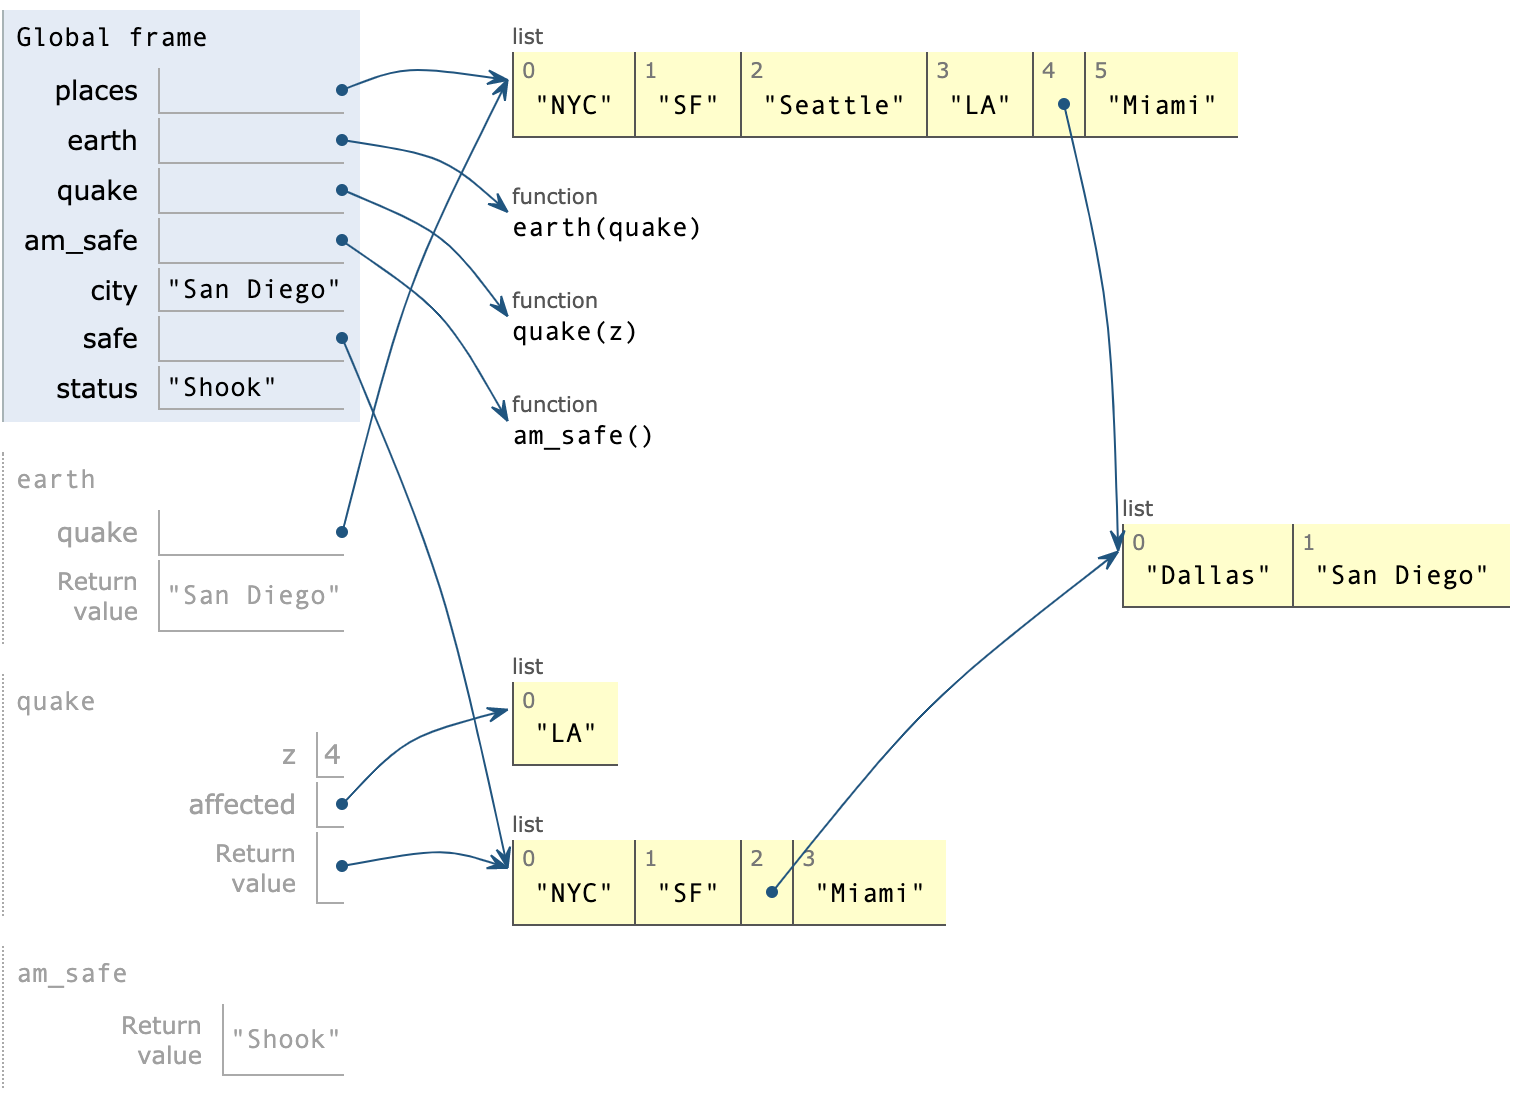
\includegraphics[width= 12cm]{rev-env.png}
\begin{lstlisting}
places = ['NYC', 'SF', 'Seattle']
def earth(quake):
    quake.extend(['LA'])
    ____(1)____
    return ____(2)____
    
def quake(z):
    affected = places[3:z]
    return ____(3)____
    
def am_safe():
    if ___(4)___:
        return 'Nothing Happened!'
    else:
        return 'Shook'
        
city = earth(places)
places += ['Miami']
safe = quake(___(5)___)
status = am_safe()
\end{lstlisting}

\textbf{Blank 1}
\begin{itemize}
    \item quake.extend(['Dallas', 'San Diego'])
    \item quake[4] = ['Dallas', 'San Diego']
    \item quake.append(['Dallas', 'San Diego'])
\end{itemize}
\begin{solution}[.25in]
\begin{itemize}
    \item quake.extend(['Dallas', 'San Diego'])
    \item quake[4] = ['Dallas', 'San Diego']
    \item[$\blacksquare$] quake.append(['Dallas', 'San Diego'])
\end{itemize}
\end{solution}

\textbf{Blank 2}
\newline
\begin{itemize}
    \item quake[-1]1]
    \item quake[4][0]
    \item quake[4][1]
    \item quake[4]
\end{itemize}

\begin{solution}[.25in] 
\begin{itemize}
    \item[$\blacksquare$] quake[-1]1]
    \item quake[4][0]
    \item[$\blacksquare$] quake[4][1]
    \item quake[4]
\end{itemize}
\end{solution}

\textbf{Blank 3}
\newline
\begin{itemize}
    \item places[:3]
    \item places[:2] + places[-2:]
    \item places[:2].append(places[4:])
\end{itemize}
\begin{solution}[.25in]
\begin{itemize}
    \item places[:3]
    \item[$\blacksquare$] places[:2] + places[-2:]
    \item places[:2].append(places[4:])
\end{itemize}
\end{solution}

\textbf{Blank 4}
\newline
\begin{itemize}
    \item city in safe
    \item city in safe[2]
    \item city not in safe[2]
\end{itemize}
\begin{solution}[.25in]
\begin{itemize}
    \item[$\blacksquare$] city in safe
    \item city in safe[2]
    \item[$\blacksquare$] city not in safe[2]
\end{itemize}\end{solution}

\textbf{Blank 5}
\newline
\begin{itemize}
    \item 3
    \item 4
    \item len(places) - 2
\end{itemize}
\begin{solution}[.25in]
\begin{itemize}
    \item 3
    \item[$\blacksquare$] 4
    \item[$\blacksquare$] len(places) - 2
\end{itemize}
\end{solution}